\section{Лекція 14: Об’єкти та класи}
\subsection{Функція isinstance} 
\begin{frame}
Функція \texttt{isinstance(obj, type)} перевіряє чи належить об'єкт \texttt{obj} до типу даних \texttt{type} і повертає \texttt{True} або \texttt{False}. Замість \texttt{type} можна використовувати кортеж із декількох типів даних.

Тип \texttt{bool} успадковується від типу \texttt{int}, тому ця функція показує, що значення \texttt{True} або \texttt{False} належать до типу \texttt{int}.

Перевірку типу даних також можна робити за допомогою функції \texttt{type}:

\texttt{type(a) == int} або \texttt{type(a) in (int, float)}  


% \frametitle{Створення рядків в Python}
\end{frame}

\subsection{Вступ до ООП} 

\begin{frame}
ООП - об'єктно орієнтоване програмування. В програмах ми оперуємо об'єктами даних.

Класи та об'єкти класів.

Клас містить властивості та методи.

Дані та методи класу можна приховувати. Інкапсуляція.

Успадкування. Властивості та методи успадковуються класами від базових класів. Дочірні класи розширюють функціональність базових.

Поліморфізм - можливість через единий інтерфейс працювати з об'єктами різних класів.
\end{frame}

\subsection{Класи та їх атрибути} 
\begin{frame}
Визначення класу.
Name - назва класу, attr\_1 та attr\_2 - атрибути класу. 

\texttt{class Name:}

\texttt{~~~~attr\_1}

\texttt{~~~~attr\_2}

 Фактично клас створює простір імен з назвою Name. Атрибути класу можна знайти в словнику \texttt{Name.\_\_dict\_\_}. Створення екземпляра класу \texttt{a = Name()}.
 
 \texttt{Name.\_\_doc\_\_} - містить рядок з описом класу.
\end{frame}

\begin{frame}
\begin{itemize}
  \item \texttt{Name.attr = val} - додає до класу \texttt{Name} атрибут \texttt{attr} зі значенням \texttt{val}.
  \item \texttt{obj.attr = val} - додає до екземпляру класу \texttt{obj} атрибут \texttt{attr} зі значенням \texttt{val}.
  \item \texttt{setattr(Name, 'attr', val)} - додає до класу \texttt{Name} атрибут \texttt{attr} зі значенням \texttt{val}.
  \item \texttt{Name.attr} - читає атрибут \texttt{attr} класу \texttt{Name}, якщо такий атрибут відсутній видає помилку.
  \item \texttt{getattr(Name, 'attr', val)} - читає атрибут \texttt{attr}  класу \texttt{Name}, якщо такий атрибут відсутній видає \texttt{val}.
\end{itemize}

\end{frame}

\begin{frame}
\begin{itemize}
  \item \texttt{del Name.attr} - видаляє з класу \texttt{Name} атрибут \texttt{attr}, якщо атрибут відсутній видає помилку.
   \item \texttt{delattr(Name, 'attr')} - видаляє з класу \texttt{Name} атрибут \texttt{attr}, якщо атрибут відсутній видає помилку.
  \item \texttt{hasattr(Name, 'attr')} - перевіряє чи є в класі \texttt{Name} атрибут \texttt{attr}.
\end{itemize}
Для об'єкту класа спочатку атрибут шукається в поточному просторі імен, а потім в просторі імен класу.
\end{frame}

\subsection{Методи класів} 
\begin{frame}
Методи - це якісь дії. Як викликати метод ?

Праметр \texttt{self} дозволяє дізнатися, з яким із екземплярів класу працює метод.

Викликати метод \texttt{set} для екземпляра \texttt{obj} класа \texttt{Name} можна так: \texttt{Name.set(obj)} або \texttt{obj.set()}.
\end{frame}

\subsection{Ініціалізатор та фіналізатор} 
\begin{frame}
Магічні методи розпочинаються та закінчуються двома символами підкреслення.

\texttt{\_\_init\_\_(self)} - викликається відразу після створення класу.

\texttt{\_\_del\_\_(self)} (фіналізатор) - викликається безпосередньо перед видаленням класу. 

У Python є збирач сміття, який видаляє об'єкти щойно вони стають непотрібними.

\end{frame}

\subsection{Магічний метод \_\_new\_\_. Паттерн Singleton} 
\begin{frame}
\texttt{\_\_new\_\_} - викликається перед створенням класу, поваертає адресу нового створеного об'єкту. 

\texttt{def \_\_new\_\_(cls, *args, **kwargs):} 

\texttt{~~~~якісь команди} 

\texttt{~~~~return super().\_\_new\_\_(cls)} 

\texttt{cls} посилається на поточний екземпляр класу. \texttt{super()} - посилається на базовий клас.

\end{frame}

\begin{frame}
Паттерн Singleton - екземпляр класу в кожний момент часу повинен бути лише один.

Прикдад для класу Name:

\texttt{\_\_instance = None}
 
\texttt{def \_\_new\_\_(cls, *args, **kwargs):} 

\texttt{~~~~if cls.\_\_instance is None:} 

\texttt{~~~~~~~~cls.\_\_instance = super().\_\_new\_\_(cls)} 

\texttt{~~~~return cls.\_\_instance} 

\texttt{def \_\_del\_\_(self):} 

\texttt{~~~~Name.\_\_instance = None}
\end{frame}

\begin{frame}
Метод класу об'явлюється за допомогою декоратора \texttt{@classmethod}, як обов'язковий аргумент приймає посилання на поточний екземпляр класу \texttt{cls}. Приклад:

\texttt{@classmethod}

\texttt{def method(cls, args):}

\texttt{~~~~some operations}

Метод класу працює з атрибутами класу, але не може звертатися до атрибутів екземпляра класу. Виклик метода класа:

\texttt{Name.method(arg)}
\end{frame}

\begin{frame}
Статичні методи не мають доступу ні до атрибутів класу, ні до атрибутів його екземпляра. Вони об'явлюються за допомогою декоратора \texttt{@staticmethod}. Використовується для створення незалежних сервісних функцій всередині класу.  
\end{frame}

\subsection{Об'єкт \texttt{property} та декоратор \texttt{@property}} 
\begin{frame}
class Name():

~~~~def \_\_init\_\_(self, p):

~~~~~~~~self.\_\_p = p

~~~~def set\_p(self, p):

~~~~~~~~self.\_\_p = p

~~~~def get\_p(self):

~~~~~~~~return self.\_\_p

~~~~p = property(get\_p, set\_p)

n = Name(val)

n.p = val1

print(n.p)
\end{frame}

\begin{frame}
class Name():

~~~~def \_\_init\_\_(self, p):

~~~~~~~~self.\_\_p = p

~~~~def set\_p(self, p):

~~~~~~~~self.\_\_p = p

~~~~def get\_p(self):

~~~~~~~~return self.\_\_p

~~~~p = property()

~~~~p = p.setter(set\_p)

~~~~p = p.getter(get\_p)

\end{frame}

\begin{frame}
class Name():

~~~~def \_\_init\_\_(self, p):

~~~~~~~~self.\_\_p = p

~~~~@property

~~~~def p(self, p):

~~~~~~~~return self.\_\_p

~~~~@p.setter

~~~~def p(self):

~~~~~~~~self.\_\_p = p

~~~~@p.deleter

~~~~def p(self):

~~~~~~~~del self.\_\_p

\end{frame}

\subsection{Успадкування} 
\begin{frame}
\begin{figure}
\begin{center}
 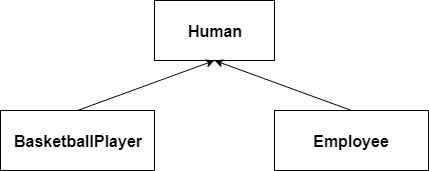
\includegraphics[width=0.4\textwidth]{pictures/inheritance.jpg}
\caption{успадкування}
\label{inheritance} 
\end{center}
\end{figure}

На малюнку \texttt{Human} - базовий або батьківський клас, а \texttt{BasketballPlaeyr} та \texttt{Employee} - підкласи або дочірні класи.

\end{frame}

\begin{frame}

Відкриті атрибути батьківського класу є доступними із класів-спадкоємців. Коли викликається метод для дочірнього класу, то спочатку він шукається в поточному класі, а потім (якщо його не знайдено) - в батьківському класі. 

Параметр в базових класах може посилатися не тільки на об'єкти поточного класу (перевизначені атрибути та методи), а й на об'єкти дочірніх класів.  

\end{frame}

\begin{frame}

\texttt{class Name:}

\texttt{~~~~def \_\_init\_\_(self):}

\texttt{~~~~~~~~pass}

\texttt{class Subname(Name):}

\texttt{~~~~def \_\_init\_\_(self):}

\texttt{~~~~~~~~super().\_\_init\_\_()}
 
Функція \texttt{super()} посилається на об'єкт базового класу. Виклик методів базового класу через функцію \texttt{super()}  називається \underline{делегування}.
\end{frame}
